
%%%%%%%%%%%%%%%%%%%%%%%%%%%%%%%%%%%%%%%%%
% Short Sectioned Assignment LaTeX Template Version 1.0 (5/5/12)
% This template has been downloaded from: http://www.LaTeXTemplates.com
% Original author:  Frits Wenneker (http://www.howtotex.com)
% License: CC BY-NC-SA 3.0 (http://creativecommons.org/licenses/by-nc-sa/3.0/)
%%%%%%%%%%%%%%%%%%%%%%%%%%%%%%%%%%%%%%%%%

%----------------------------------------------------------------------------------------
%	PACKAGES AND OTHER DOCUMENT CONFIGURATIONS
%----------------------------------------------------------------------------------------

\documentclass[paper=a4, fontsize=11pt]{scrartcl} % A4 paper and 11pt font size

% ---- Entrada y salida de texto -----

\usepackage[T1]{fontenc} % Use 8-bit encoding that has 256 glyphs
\usepackage[utf8]{inputenc}
%\usepackage{fourier} % Use the Adobe Utopia font for the document - comment this line to return to the LaTeX default

% ---- Idioma --------

\usepackage[spanish, es-tabla]{babel} % Selecciona el español para palabras introducidas automáticamente, p.ej. "septiembre" en la fecha y especifica que se use la palabra Tabla en vez de Cuadro

% ---- Otros paquetes ----

\usepackage{url} % ,href} %para incluir URLs e hipervínculos dentro del texto (aunque hay que instalar href)
\usepackage{amsmath,amsfonts,amsthm} % Math packages
%\usepackage{graphics,graphicx, floatrow} %para incluir imágenes y notas en las imágenes
\usepackage{graphics,graphicx, float} %para incluir imágenes y colocarlas
\usepackage{subfigure} % subfiguras

% Para hacer tablas comlejas
%\usepackage{multirow}
%\usepackage{threeparttable}

%\usepackage{sectsty} % Allows customizing section commands
%\allsectionsfont{\centering \normalfont\scshape} % Make all sections centered, the default font and small caps

\usepackage{fancyhdr} % Custom headers and footers
\usepackage{pdflscape}

\pagestyle{fancyplain} % Makes all pages in the document conform to the custom headers and footers
\fancyhead{} % No page header - if you want one, create it in the same way as the footers below
\fancyfoot[L]{} % Empty left footer
\fancyfoot[C]{} % Empty center footer
\fancyfoot[R]{\thepage} % Page numbering for right footer
\renewcommand{\headrulewidth}{0pt} % Remove header underlines
\renewcommand{\footrulewidth}{0pt} % Remove footer underlines
\setlength{\headheight}{13.6pt} % Customize the height of the header

\numberwithin{equation}{section} % Number equations within sections (i.e. 1.1, 1.2, 2.1, 2.2 instead of 1, 2, 3, 4)
\numberwithin{figure}{section} % Number figures within sections (i.e. 1.1, 1.2, 2.1, 2.2 instead of 1, 2, 3, 4)
\numberwithin{table}{section} % Number tables within sections (i.e. 1.1, 1.2, 2.1, 2.2 instead of 1, 2, 3, 4)


\setlength\parindent{0pt} % Removes all indentation from paragraphs - comment this line for an assignment with lots of text

\newcommand{\horrule}[1]{\rule{\linewidth}{#1}} % Create horizontal rule command with 1 argument of height
\usepackage[breaklinks=true]{hyperref}

\usepackage[dvipsnames]{xcolor}
\usepackage{amssymb}
\usepackage{color}
\usepackage{listings}
\usepackage{upgreek} % para poner letras griegas sin cursiva
\usepackage{cancel} % para tachar
\usepackage{mathdots} % para el comando \iddots
\usepackage{mathrsfs} % para formato de letra
\usepackage{stackrel} % para el comando \stackbin
\lstset{ %
language=C++,                % elegir el lenguaje del código
stringstyle=\color{blue}\ttfamily,,
basicstyle=\normalsize\ttfamily,       % el tamaño del font a usar para el código
numbers=left,                   % dónde poner los números de línea 
numberstyle=\footnotesize,      % tamaño de font usados para los números de línea 
stepnumber=1,                   % el paso de numeración
numbersep=5pt,                  % distancia del numero de línea y la línea
backgroundcolor=\color{white},  % color de fondo, para usarlo hay que agregar  \usepackage{color}
showspaces=false,               % mostrar espacios en blanco ?
showstringspaces=false,         % subrayar espacios con cadenas?   
 showtabs=false,                 % mostrar taba usando cadenas? 
frame=single,           			% enmarcar el código?  
tabsize=2,          				% sets default tabsize to 2 spaces?
keywordstyle=\color{MidnightBlue}\ttfamily\bfseries,
commentstyle=\color{OliveGreen}\ttfamily,
morecomment=[l][\color{OliveGreen}]{\#},
captionpos=b,           % sets the caption-position to bottom?
breaklines=true,        % sets automatic line breaking?
breakatwhitespace=false,    % sets if automatic breaks should only happen at whitespace ?
title=\lstname,
escapeinside={\%*}{*)}          % if you want to add a comment within your code
}

\lstset{literate=
  {á}{{\'a}}1 {é}{{\'e}}1 {í}{{\'i}}1 {ó}{{\'o}}1 {ú}{{\'u}}1
  {Á}{{\'A}}1 {É}{{\'E}}1 {Í}{{\'I}}1 {Ó}{{\'O}}1 {Ú}{{\'U}}1
  {à}{{\`a}}1 {è}{{\`e}}1 {ì}{{\`i}}1 {ò}{{\`o}}1 {ù}{{\`u}}1
  {À}{{\`A}}1 {È}{{\'E}}1 {Ì}{{\`I}}1 {Ò}{{\`O}}1 {Ù}{{\`U}}1
  {ä}{{\"a}}1 {ë}{{\"e}}1 {ï}{{\"i}}1 {ö}{{\"o}}1 {ü}{{\"u}}1
  {Ä}{{\"A}}1 {Ë}{{\"E}}1 {Ï}{{\"I}}1 {Ö}{{\"O}}1 {Ü}{{\"U}}1
  {â}{{\^a}}1 {ê}{{\^e}}1 {î}{{\^i}}1 {ô}{{\^o}}1 {û}{{\^u}}1
  {Â}{{\^A}}1 {Ê}{{\^E}}1 {Î}{{\^I}}1 {Ô}{{\^O}}1 {Û}{{\^U}}1
  {œ}{{\oe}}1 {Œ}{{\OE}}1 {æ}{{\ae}}1 {Æ}{{\AE}}1 {ß}{{\ss}}1
  {ű}{{\H{u}}}1 {Ű}{{\H{U}}}1 {ő}{{\H{o}}}1 {Ő}{{\H{O}}}1
  {ç}{{\c c}}1 {Ç}{{\c C}}1 {ø}{{\o}}1 {å}{{\r a}}1 {Å}{{\r A}}1
  {€}{{\EUR}}1 {£}{{\pounds}}1
  {ñ}{{\~n}}1
}

\hypersetup{
    colorlinks=true,
    linkcolor=black,
    filecolor=magenta,      
    urlcolor=blue,
    pdftitle={EC: Práctica 3 - Mario Rodríguez Ruiz},
    bookmarks=true,
    citecolor=blue,
}



%----------------------------------------------------------------------------------------
%	TÍTULO Y DATOS DEL ALUMNO
%----------------------------------------------------------------------------------------

\title{	
\normalfont \normalsize 
\textsc{\textbf{Estructura de Computadores (2016-2017)} \\ Subgrupo C3 \\ Grado en Ingeniería Informática\\ Universidad de Granada} \\ [25pt] % Your university, school and/or department name(s)
\horrule{0.5pt} \\[0.4cm] % Thin top horizontal rule
\huge Práctica 3: Programación	mixta	C-asm	x86	Linux \\ % The assignment title
\horrule{2pt} \\[0.5cm] % Thick bottom horizontal rule
}

\author{Mario Rodríguez Ruiz} % Nombre y apellidos

\date{\normalsize\today} % Incluye la fecha actual

%----------------------------------------------------------------------------------------
% DOCUMENTO
%----------------------------------------------------------------------------------------

\begin{document}

\maketitle % Muestra el Título

\newpage %inserta un salto de página

\tableofcontents % para generar el índice de contenidos

\listoffigures

\newpage

%----------------------------------------------------------------------------------------
%	Diario de trabajo
%----------------------------------------------------------------------------------------
\section{Diario de trabajo}
\subsection {Primera sesión}
Finalizar el tutorial de la práctica 3. 
Ejecutar las distintas versiones del programa \textbf{suma}:

La primera versión consistía en modificar el código para que funcionara
según \textbf{cdecl}.

La segunda añadía la llamada \textbf{printf()} para sacar por pantalla el 
resultado en decimal y hexadecimal que sustituye la llamada directa al kernel Linux.

La tercera eliminaba cualquier rastro de ensamblador en \textbf{suma()} creando una nueva equivalencia completa en \textbf{C}.

La cuarta dejaba como única instrucción un salto a la subrutina suma.

La quinta era dejar completamente el código en \textbf{lenguaje C}.

La sexta consistía en volver a pasar la función suma a un módulo ensamblador separado.

En la séptima se volvía a incorporar el código ensamblador de suma como ensamblador en-linea.

La octava versión reducía el código ensamblador en-linea al cuerpo del bucle \textbf{for}.

Y por último, en la novena se creaban \textbf{tres alternativas a suma} cronometrando sus tiempos de ejecución.

\subsection {Segunda sesión}
Realización de las preguntas de autocomprobación desde suma\_01 hasta suma\_09.

Estudio de las distintas versiones de \textbf{popcount} a realizar así
como una pequeña estructuración y organización de cada uno de ellos.

Desarrollo de cada uno de los códigos correspondientes a \textbf{popcount}, por medio
del guión de prácticas con la ayuda de las transparencias de clase y del libro de la asignatura
para llegar a sus soluciones.

Toma de los resultados obtenidos en las ejecuciones y elaboración de un estudio por 
medio de una hoja de cálculo con sus correspondientes gráficas finales.

\subsection {Tercera sesión}

Estudio de las distintas versiones de \textbf{parity} a realizar así
como una pequeña estructuración y organización de cada uno de ellos.

Desarrollo de cada uno de los códigos correspondientes a \textbf{parity}, por medio
del guión de prácticas con la ayuda de las transparencias de clase y del libro de la asignatura
para llegar a sus soluciones.

Toma de los resultados obtenidos en las ejecuciones y elaboración de un estudio por 
medio de una hoja de cálculo con sus correspondientes gráficas finales.

\newpage
%----------------------------------------------------------------------------------------
%	Ejercicio 4.0
%----------------------------------------------------------------------------------------

\section{Ejercicio 4.0: Preguntas de autocomprobación (suma\_01-suma\_09)}
\subsection{Sesión de depuración suma\_01\_S\_cdecl}
\textbf{\textit{4.¿Qué modos de direccionamiento usa la instrucción add (\%ebx,\%edx,4), \%eax?}}
\\

La instrucción usa el modo de direccionamiento inmediato.

Los componentes son: add(rt, rs, imm),escala.

\subsection{Sesión de depuración suma\_02\_S\_libC}
\textbf{\textit{1.¿Qué error se obtiene si no se añade –lc al comando de enlazar? ¿Qué tipo de error es? (en tiempo de ensamblado, enlazado, ejecución...)
}}
\\

Se obtienen varios errores de referencias a funciones que no están definidas.

Se trata de un error en tiempo de enlazado.

\subsection{Sesión de depuración suma\_03\_SC}
\textbf{\textit{2.¿Qué diferencia hay entre los comandos Next y Step?}}
\\

La diferencia está en que, por ejemplo, si se encuentra en una llamada a función y se ejecuta el comando \textbf{Next}, la función se ejecutará y volverá. En cambio con \textbf{Step} se irá a la primera línea de esa función.


\subsection{Sesión de depuración suma\_04\_SC}
\textbf{\textit{3. Otras diferencias están en el manejo de pila. Explicar dichas diferencias.}}
\\

La función \textbf{\_\_printf\_chk flag} comprobará el desbordamiento de pila antes de calcular un resultado, dependiendo del valor del parámetro \textit{flag}. Si se prevé un desbordamiento, la función se cancelará y el programa se saldrá del programa que la llama.

\subsection{Sesión de depuración suma\_05\_SC}
\textbf{\textit{5. Se aplica una máscara 
		al punte ero de pila. ¿Cuál, 
		y  qué efecto produce? (Pista: alineamiento). 
		Nosotros usam
		mos .int para de clarar enteros y arrays. ¿Qué usa 
		gcc? Nosotros usamos el contador de posiciones y aritmé
		ética de etiquetas para calcular la longitud del array. ¿Qué usa gcc? Nosotros hemos usado push para introducir argumentos en pila, ¿Cuál usa gcc? 
}}
\\

Máscara de pila: \textbf{leaq	0(,\%rax,4), \%rdx}

Para declarar enteros y arrays gcc usa \textbf{.long}

gcc para introducir argumentos en pila utiliza \textbf{pushq}

\subsection{Sesión de depuración suma\_07\_Casm}
\textbf{\textit{Por motivos estéticos, a veces se terminan las líneas ASM con $ "\textbackslash n" $ y otras con $ "\textbackslash n \textbackslash t" $.  
		¿Por qué en este caso apenas se ha usado $ "\textbackslash t" $?}}
	\\
	
	No se ha usado apenas $ "\textbackslash t" $ para que cuando se imprima el código para su depuración o para su lectura resulte más cómodo.

\subsection{Sesión de depuración suma\_08\_Casm}
\textbf{\textit{Si res es variable de salida, ¿por qué se le ha indicado restricción $ "+r" $, en lugar de $ "=r" $? 
}}
\\

Se le ha indicado la restricción $ "+r" $ porque ésta le dice a gcc qué necesita para cargar un registro con el valor, es decir, significa que este operando es leído y escrito por la instrucción.

Cuando el compilador arregla los operandos para satisfacer las restricciones, necesita saber qué operandos son leídos por la instrucción y que son cuáles por ella. \textbf{'='} Identifica un operando que solamente se encuentra escrito, sin embargo \textbf{'+'} identifica un operando que es escrito y a la vez leído.

\newpage

\section{Ejercicio 4.1: Calcular la suma de bits de una lista de enteros sin signo}
\subsection{Primera versión}
\begin{lstlisting}
// Primera versión, previsiblemente con peores prestaciones.
int popcount1(unsigned* array, int len)
{
	int  i,j,  res=0;
	for (i=0; i<len; i++){
		unsigned x =array[i];
		for (j=0; j<WSIZE;j++){     // Recorre los bits
			res += x & 0x1;         	// Aplica la máscara 0x1
			x >>=1;                 	// Desplaza a la derecha
		}
	}
	return res;
}
\end{lstlisting}

\subsection{Segunda versión}
\begin{lstlisting}
int popcount2(unsigned* array, int len)
{
	int  i, res=0;
	unsigned x;
	for (i=0; i<len; i++){
		x=array[i];
		do{
			res += x & 0x1;         // Aplica la máscara 0x1
			x >>=1;                 // Desplaza a la derecha
		}while(x);                // Recorre los bits
	}
	return res;
}
\end{lstlisting}

\newpage

\subsection{Tercera versión}
\begin{lstlisting}
// Traduce el bucle interno while por código ASM.
int popcount3(unsigned* array, int len){
	int res=0,i;
	unsigned x;
	
	for(i=0; i<len; i++){
		x=array[i];
		asm("\n"
			"ini3:		\n\t"        // seguir mientras que x!=0
			"shr %[x]	\n\t"        // LSB en CF
			"adc $0, %[r] \n\t"    // suma con acarreo
			"cmp $0,%[x] \n\t"     // compara
			"jne	ini3 \n\t"       // salto, modificando CF y ZF
			: [r]"+r" (res)        // e/s: añadir a lo acumulado por el momento
			: [x]"r" (x)           // entrada: valor elemento
		);
	}
	return res;
}
\end{lstlisting}

\subsection{Cuarta versión}
\begin{lstlisting}
int popcount4(unsigned* array, int len){
	int i,j;
	int result = 0;
	unsigned n;
	
	for(i = 0; i < len; i++){
		int res = 0;
		n = array[i];
		for(j = 0; j < 8; j++){     // Aplica la máscara a cada elemento.
			res += n & 0x01010101;    // Acumula los bits de cada byte.
			n >>= 1;
		}
		// Suma en árbol los 4B
		res += (res >> 16);
		res += (res >> 8);
		result += (res & 0xff);
	}
	return result;
}
\end{lstlisting}

\subsection{Quinta versión}
\begin{lstlisting}
// Versión SSSE3 (pshufb)
int popcount5(unsigned* array, int len) {
	int i;
	int res, result = 0;
	int SSE_mask[] = { 0x0f0f0f0f, 0x0f0f0f0f, 0x0f0f0f0f, 0x0f0f0f0f };
	int SSE_LUTb[] = { 0x02010100, 0x03020201, 0x03020201, 0x04030302 };
	
	if (len & 0x3)
		printf("leyendo 128b pero len no múltiplo de 4?n");
	for (i = 0; i < len; i += 4) {
		asm("movdqu        %[x], %%xmm0 \n\t"
		"movdqa  %%xmm0, %%xmm1 \n\t"       // dos copias de x
		"movdqu    %[m], %%xmm6 \n\t"       // máscara
		"psrlw           $4, %%xmm1 \n\t"
		"pand    %%xmm6, %%xmm0 \n\t"       // xmm0 - nibbles inferiores
		"pand    %%xmm6, %%xmm1 \n\t"       // xmm1 - nibbles superiores
		
		"movdqu    %[l], %%xmm2 \n\t"       // como pshufb sobrescribe LUT
		"movdqa  %%xmm2, %%xmm3 \n\t"       // queremos 2 copias
		"pshufb  %%xmm0, %%xmm2 \n\t"       // xmm2 = vector popcount inferiores
		"pshufb  %%xmm1, %%xmm3 \n\t"       // xmm3 = vector popcount superiores
		
		"paddb   %%xmm2, %%xmm3 \n\t"       // xmm3 - vector popcount bytes
		"pxor    %%xmm0, %%xmm0 \n\t"       // xmm0 = 0,0,0,0
		"psadbw  %%xmm0, %%xmm3 \n\t"       // xmm3 = [pcnt bytes0..7|pcnt bytes8..15]
		"movhlps %%xmm3, %%xmm0 \n\t"       // xmm3 = [       0      |pcnt bytes0..7 ]
		"paddd   %%xmm3, %%xmm0 \n\t"       // xmm0 = [   no usado   |pcnt bytes0..15]
		"movd    %%xmm0, %[res] \n\t"
		: [res]"=r" (res)
		: [x]  "m"  (array[i]),
		[m]  "m"  (SSE_mask[0]),
		[l]  "m"  (SSE_LUTb[0])
		);
		result += res;
	}
	return result;
}
\end{lstlisting}

\subsection{Sexta versión}
\begin{lstlisting}
// Versión SS4.2
int popcount6(unsigned* array, int len) {
	int i;
	unsigned x;
	int val, result=0;
	
	for(i=0; i<len; i++){
		x=array[i];
		asm("popcnt %[x], %[val]"
		: [val] "=r" (val)
		:   [x]  "r" (x)
		);
		result += val;
	}
	return result;
}
\end{lstlisting}

\newpage

\subsection{Mediciones:	cronometrar las	distintas versiones con	-O0, -O1 y -O2}



\begin{figure}[H] %con el [H] le obligamos a situar aquí la figura
	\centering
	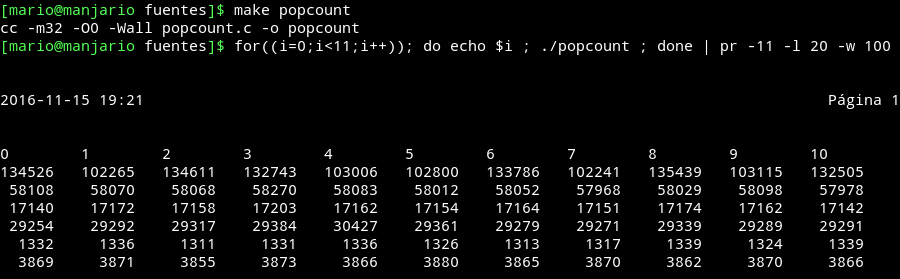
\includegraphics[scale=0.6]{capturas/ej0_pop.png} 
	\caption{Ejecución del programa \textbf{popcount} con \textbf{-O0}} 
	\label{fig:figura2}
\end{figure}

\begin{figure}[H] %con el [H] le obligamos a situar aquí la figura
	\centering
	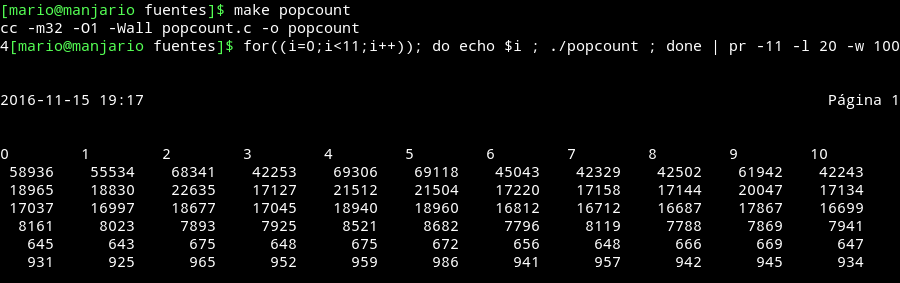
\includegraphics[scale=0.6]{capturas/ej1_pop.png} 
	\caption{Ejecución del programa \textbf{popcount} con \textbf{-O1}} 
	\label{fig:figura3}
\end{figure}

\begin{figure}[H] %con el [H] le obligamos a situar aquí la figura
	\centering
	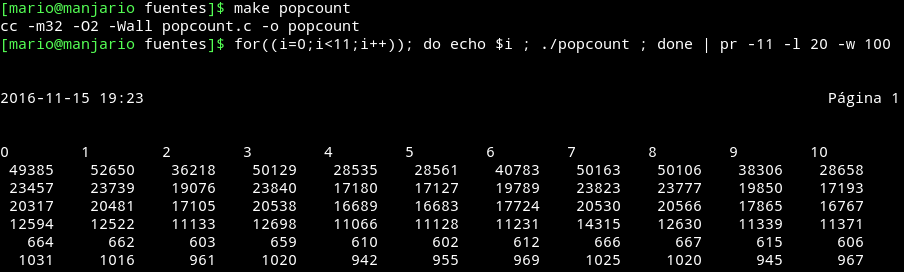
\includegraphics[scale=0.6]{capturas/ej2_pop.png} 
	\caption{Ejecución del programa \textbf{popcount} con \textbf{-O2}} 
	\label{fig:figura4}
\end{figure}

\newpage

\subsection{Representación de los resultados}
\begin{figure}[H] %con el [H] le obligamos a situar aquí la figura
	\centering
	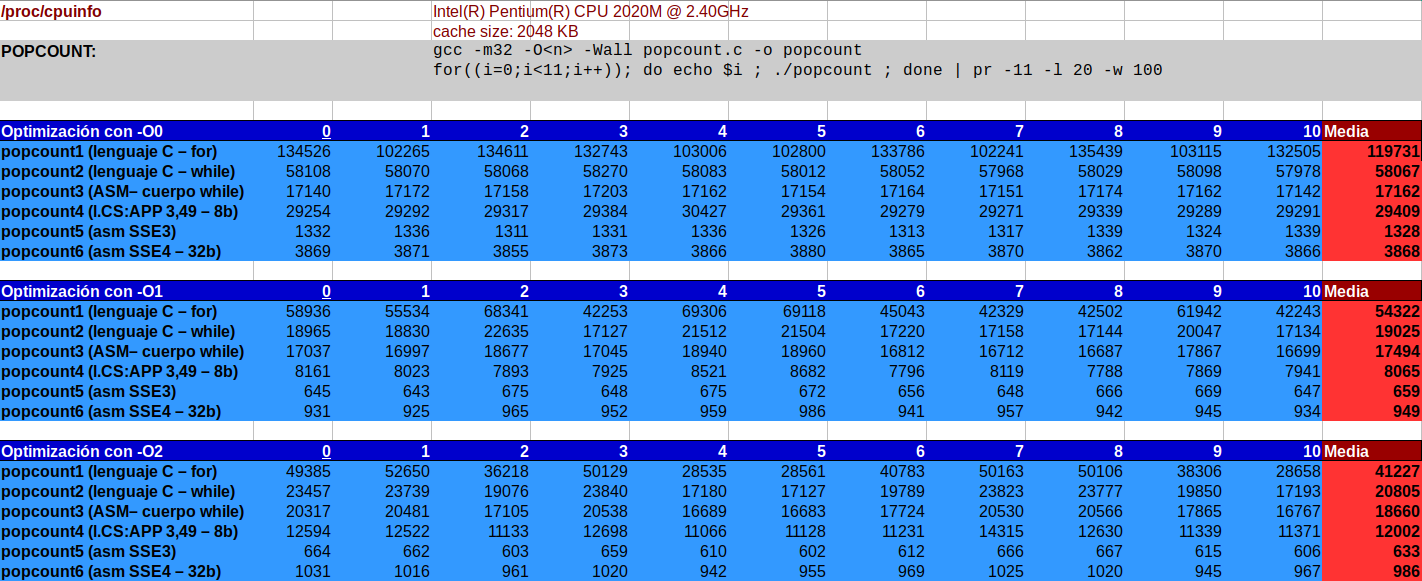
\includegraphics[scale=0.4]{capturas/tablas_pop.png} 
	\caption{Resultado de las ejecuciones de \textbf{popcount}} 
	\label{fig:figura5}
\end{figure}

\begin{figure}[H] %con el [H] le obligamos a situar aquí la figura
	\centering
	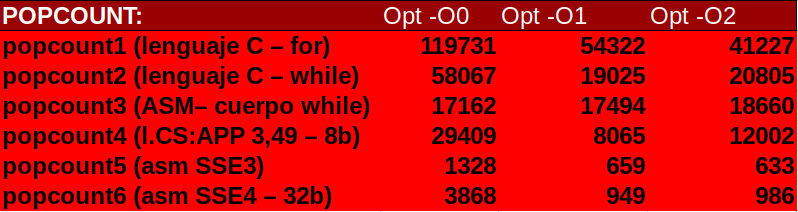
\includegraphics[scale=0.6]{capturas/medias_pop.png} 
	\caption{Resumen de los promedios} 
	\label{fig:figura6}
\end{figure}

\begin{figure}[htbp]
	\centering
	\subfigure[Completa]{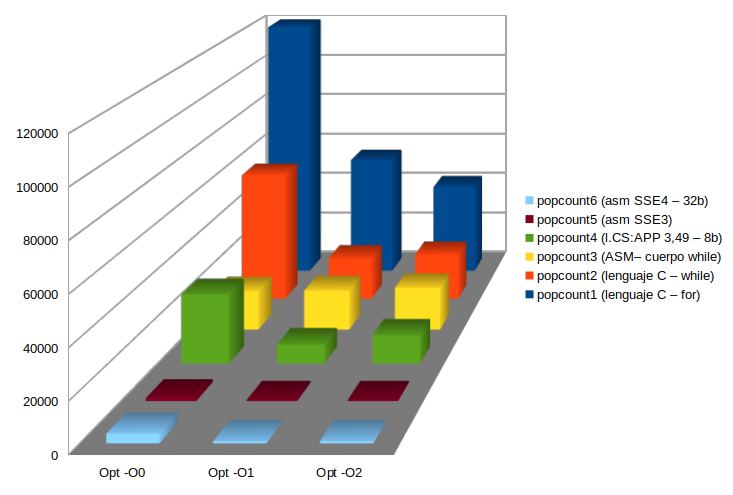
\includegraphics[scale=0.35]{capturas/graf_pop1.png}}
	\subfigure[Reducida para apreciar el factor mejora]{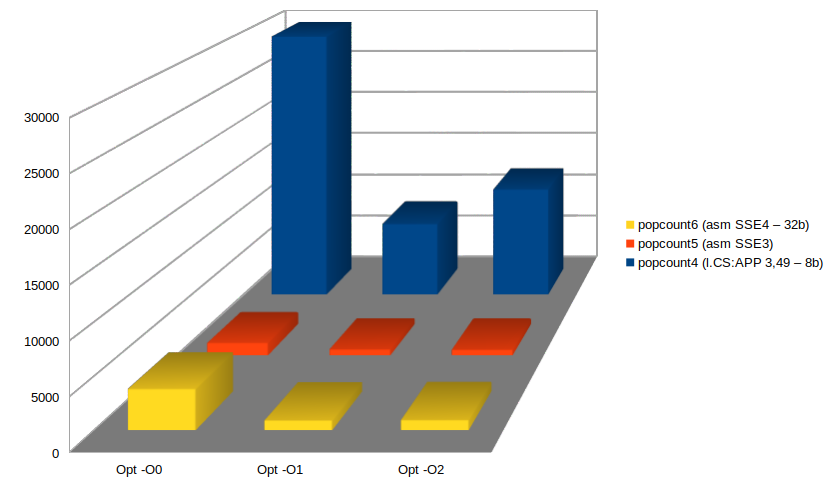
\includegraphics[scale=0.35]{capturas/graf_pop2.png}}
	\caption{Gráficas de las ejecuciones de \textbf{popcount}} \label{fig:lego}
\end{figure}


\newpage

\section{Ejercicio 4.2: Calcular la suma de paridades de una lista de entero sin signo}
\subsection{Primera versión}
\begin{lstlisting}
// Primera versión
int parity1(unsigned* array, int len)
{
	int  i,j,  res=0,val;
	for (i=0; i<len; i++){          // Recorre el array
		val=0;
		unsigned x =array[i];
		for (j=0; j<WSIZE;j++){     // Recorre los bits
			val ^= x & 0x1;         // Aplica la máscara y acumula lateralmente los bits
			x >>=1;                 // Desplaza a la derecha para extraer y acumular bits
		}
		res+=val;
	}
	return res;
}
\end{lstlisting}

\subsection{Segunda versión}
\begin{lstlisting}
// Segunda versión
int parity2(unsigned* array, int len)
{
	int  i,res=0,val;
	unsigned x;
	for (i=0; i<len; i++){
		val=0;
		x=array[i];
		do{
			val ^= x & 0x1;     // Aplica la máscara y acumula lateralmente los bits
			x >>=1;             // Desplaza a la derecha para extraer y acumular bits
		}while(x);              // Recorre el array
		res+=val;
	}
	return res;
}
\end{lstlisting}

\subsection{Tercera versión}
\begin{lstlisting}
// Tercera versión: Adapta la segunda versión para el array completo
int parity3(unsigned* array, int len) {
	int i;
	unsigned x;
	int result = 0;
	for (i = 0; i < len; i++) {
		x = array[i];
		int res=0;
		while (x) {
			res ^= x;            // Acumula lateralmente los bits
			x >>= 1;             // Desplaza a la derecha para extraer y acumular bits
		}
		result += res & 0x1;     // Aplicar la máscara al acumular con result.
	}
	return result;
}
\end{lstlisting}

\subsection{Cuarta versión}
\begin{lstlisting}
// Cuarta versión: Traduce el bucle intero por ASM
	int parity4(unsigned* array, int len) {
	int i,res;
	unsigned x;
	int result = 0;
	for (i = 0; i < len; i++) {
		x = array[i];
		res = 0;
		asm(
			"ini3:				\n\t"   // seguir mientras que x!=0
			"xor %[x], %[v]		\n\t"
			"shr $1, %[x]		\n\t"   // LSB en ZF
			"test %[x], %[x]	\n\t"
			"jnz ini3			\n\t"   // salto, modificando CF y ZF
			: [v]"+r"(res)              // e/s: entrada 0, salida paridad elemento
			
			: [x]"r"(x)                 // entrada: valor elemento
		);
		result += res & 0x1;            // Aplicar la máscara al acumular con result.
	}
	return result;
}
\end{lstlisting}

\subsection{Quinta versión}
\begin{lstlisting}
// Quinta versión: Suma en árbol
int parity5(unsigned* array, int len) {
	int i, j;
	int result = 0;
	unsigned x;
	for (i = 0; i < len; i++) {
		x = array[i];
		// Somete a cada elemento a XOR y desplazamientos
		// sucesivos a mitdad de la distancia cada vez
		for (j = 16; j > 0; j /= 2)
			x ^= x >> j;
		result += x & 0x01;     // Aplica la máscara al valor final.
	}
	return result;
}
\end{lstlisting}

\newpage

\subsection{Sexta versión}
\begin{lstlisting}
// Sexta versión: Traduce el bucle for por ASM
int parity6(unsigned* array, int len) {
	int j,result = 0;;
	unsigned x = 0;
	
	for (j = 0; j < len; j++) {
		x = array[j];
		asm(
			"mov	%[x], %%edx	     \n\t" // Sacar copia para XOR
			"shr	$16,	%%edx	 \n\t"
			"xor	%[x],	%%edx	 \n\t" // PF, señalando la paridad par de los 8 bits inferiores
			"xor	%%dh,	%%dl	 \n\t"
			"setpo  %%dl	         \n\t"
			"movzx	%%dl,	%[x]	 \n\t" // Devuelve en 32 bits
			: [x] "+r" (x)                 // e/s entrada valor elemento, salida paridad
			:
			: "edx"                        // clobber
		);
		result += x;
	}
	return result;
}
\end{lstlisting}

\newpage

\subsection{Mediciones:	cronometrar las	distintas versiones con	-O0, -O1 y -O2}



\begin{figure}[H] %con el [H] le obligamos a situar aquí la figura
	\centering
	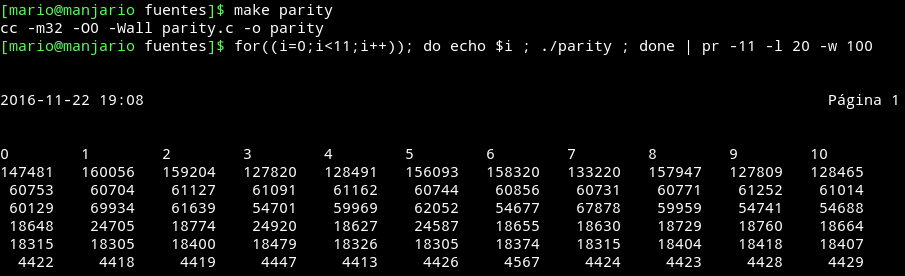
\includegraphics[scale=0.6]{capturas/ej0_par.png} 
	\caption{Ejecución del programa \textbf{parity} con \textbf{-O0}} 
	\label{fig:par1}
\end{figure}

\begin{figure}[H] %con el [H] le obligamos a situar aquí la figura
	\centering
	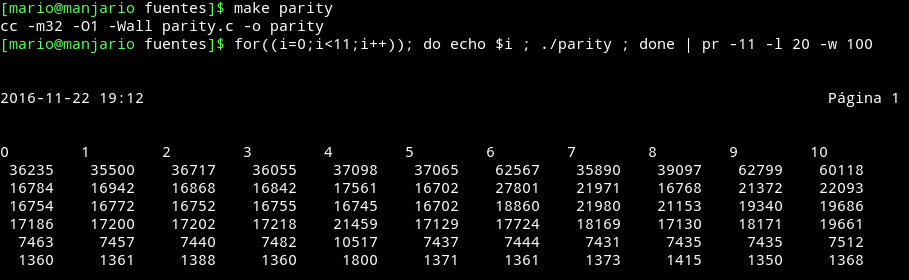
\includegraphics[scale=0.6]{capturas/ej1_par.png} 
	\caption{Ejecución del programa \textbf{parity} con \textbf{-O1}} 
	\label{fig:par3}
\end{figure}

\begin{figure}[H] %con el [H] le obligamos a situar aquí la figura
	\centering
	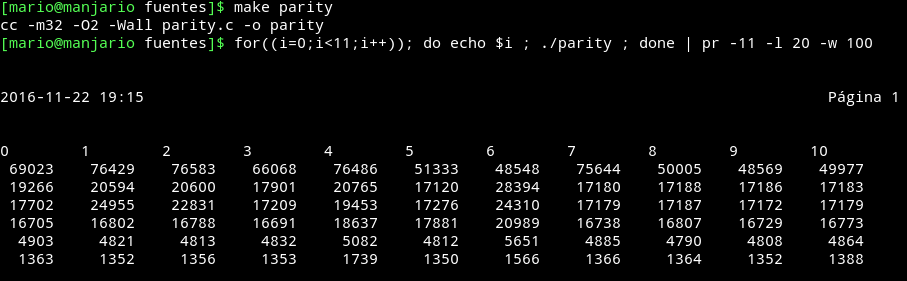
\includegraphics[scale=0.6]{capturas/ej2_par.png} 
	\caption{Ejecución del programa \textbf{parity} con \textbf{-O2}} 
	\label{fig:par4}
\end{figure}

\newpage

\subsection{Representación de los resultados}
\begin{figure}[H] %con el [H] le obligamos a situar aquí la figura
	\centering
	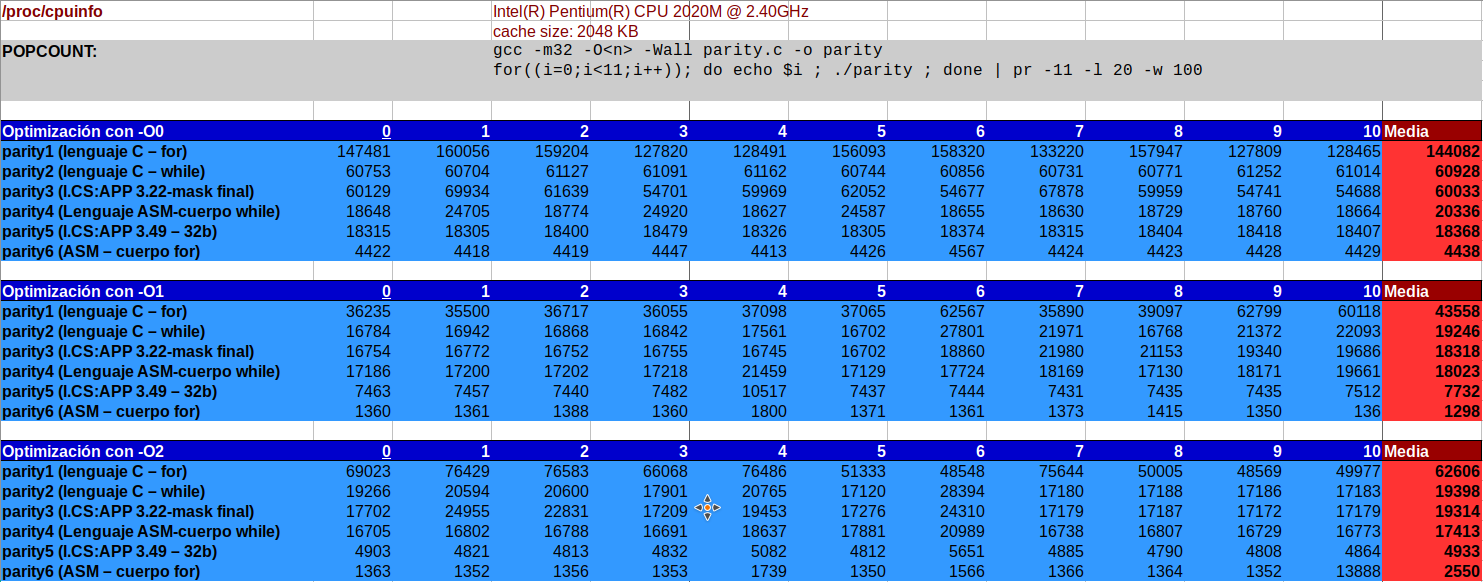
\includegraphics[scale=0.4]{capturas/tablas_par.png} 
	\caption{Resultado de las ejecuciones de \textbf{parity}} 
	\label{fig:par5}
\end{figure}

\begin{figure}[H] %con el [H] le obligamos a situar aquí la figura
	\centering
	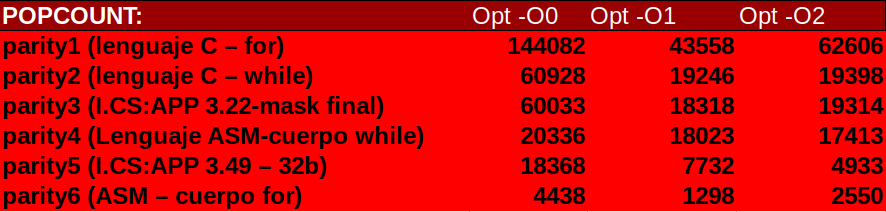
\includegraphics[scale=0.6]{capturas/medias_par.png} 
	\caption{Resumen de los promedios} 
	\label{fig:par6}
\end{figure}

\begin{figure}[htbp]
	\centering
	\subfigure[Completa]{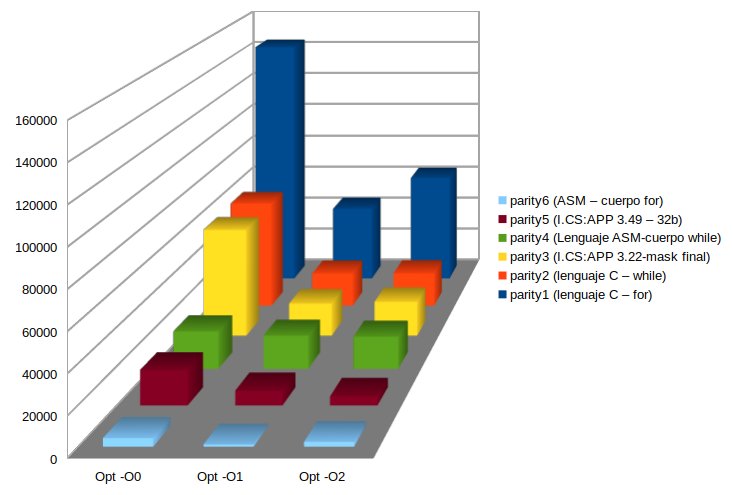
\includegraphics[scale=0.35]{capturas/graf_par2.png}}
	\subfigure[Reducida para apreciar el factor mejora]{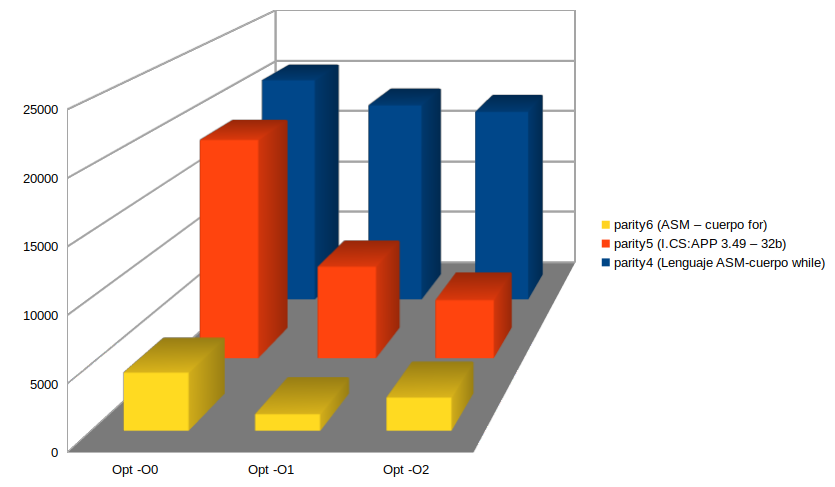
\includegraphics[scale=0.35]{capturas/graf_par1.png}}
	\caption{Gráficas de las ejecuciones de \textbf{parity}} \label{fig:par7}
\end{figure}

\newpage

\end{document}
